\documentclass{article}
\usepackage{fullpage}
\usepackage{graphicx}
\usepackage[hidelinks]{hyperref}

\usepackage{color}
\usepackage{amsmath,amssymb,amsthm}
\usepackage{natbib}

\bibliographystyle{plainnat}


\newcommand{\R}{\mathbb{R}}
\newcommand{\Q}{\mathbb{Q}}
\newcommand{\Z}{\mathbb{Z}}
\newcommand{\N}{\mathbb{N}}

\renewcommand{\P}{\mathbb{P}}
\newcommand{\E}{\mathbb{E}}
\newcommand{\var}{\mathop{\mbox{Var}}}
\newcommand{\cov}{\mathop{\mbox{cov}}}
%\newcommand{\det}{\mathop{\mbox{det}}}
\newcommand{\deg}{\mathop{\mbox{deg}}}
\newcommand{\supp}{\mathop{\mbox{supp}}}
\newcommand{\sgn}{\mathop{\mbox{sgn}}}

\newcommand{\bone}{\mathbf{1}}
\newcommand{\st}{\,\colon\,}

% These macros are borrowed from TAOCPMAC.tex
\newcommand{\slug}{\hbox{\kern1.5pt\vrule width2.5pt height6pt depth1.5pt\kern1.5pt}}
\def\xskip{\hskip 7pt plus 3pt minus 4pt}
\newdimen\algindent
\newif\ifitempar \itempartrue % normally true unless briefly set false
\def\algindentset#1{\setbox0\hbox{{\bf #1.\kern.25em}}\algindent=\wd0\relax}
\def\algbegin #1 #2{\algindentset{#21}\alg #1 #2} % when steps all have 1 digit
\def\aalgbegin #1 #2{\algindentset{#211}\alg #1 #2} % when 10 or more steps
\def\alg#1(#2). {\medbreak % Usage: \algbegin Algorithm A (algname). This...
  \noindent{\bf#1}({\it#2\/}).\xskip\ignorespaces}
\def\kalgstep#1.{\ifitempar\smallskip\noindent\else\itempartrue
   \hskip-\parindent\fi
   \hbox to\algindent{\bf\hfil #1.\kern.25em}%
   \hangindent=\algindent\hangafter=1\ignorespaces}

\newcommand{\algstep}[3]{\kalgstep #1 [#2] #3 }
\newenvironment{taocpalg}[3]{%
\vspace{1em}%
\algbegin Algorithm #1. ({#2}). #3 }
{\vspace{1em}}

\newcommand{\randomuniform}[0]{\mathcal{R}_U}
\newcommand{\randomdiscrete}[0]{\mathcal{R}_D}
\newcommand{\algref}[1]{#1}


\newcommand{\tskit}{{\texttt{tskit}}}
\newcommand{\branch}{\mbox{Branch}} % branch stat
\newcommand{\branchp}{\mbox{Branch}_+} % polarised
\newcommand{\site}{\mbox{Site}} % site stat
\newcommand{\sitep}{\mbox{Site}_+} % polarised
\newcommand{\node}{\mbox{Node}} % node stat
\newcommand{\nodep}{\mbox{Node}_+} % polarised
\newcommand{\given}{\;\vert\;}

\newcommand{\treeseq}{\mathbb{T}} % tree sequence
\newcommand{\iw}{w} % sample (initial) weights
\newcommand{\tiw}{w_\text{total}} % total sample (initial) weights
\newcommand{\nw}{x} % subtree (node) weights
\newcommand{\aw}{{\bar x}} % allele weights

\newcommand{\plr}[1]{{\color{blue}\textbf{plr:} \it #1}}
\newcommand{\jk}[1]{{\color{red}\textbf{jk:} \it #1}}


\begin{document}

\title{
    Efficiently summarising relationships in large samples:
    a general duality between statistics of genealogies and genomes}
\author{Peter Ralph, Kevin Thornton, and Jerome Kelleher}
\maketitle

% \emph{Running head:} Genealogies and genomes


%%%%%%%%%%
\section*{Abstract}

As a genetic mutation is passed down across generations,
it distinguishes those genomes that have inherited it from those that have not,
thus providing a glimpse of the genealogical tree that relates the genomes to each other at that site.
Summaries of genetic variation thus also aim to summarize the underlying genealogies.
Here we exploit this duality to create a method that efficiently computes single-site statistics
from population genetic data using the succinct tree sequence encoding
of genome sequence and genealogies.
We use the framework to provide fast implementations of many currently-defined statistics
(whose run time scales with the logarithm of the number of samples),
and to suggest several statistics.
The general approach aggregates ``sample weights'' up each marginal tree,
which are then summarised using a ``summary function'';
different statistics result from different choices of weight or function.
The results can be summarised in three different ways:
by \emph{site}, which corresponds to statistics calculated from genome sequence,
by \emph{branch}, which gives the expected value of the site statistic
with a large number of infinite-sites mutations,
or by \emph{node}, which summarises the contribution of each node in the tree to the statistics.
This formulation also makes it easy to see what statistic of the underlying genealogical trees
each sequence-based statistic is estimating.

\plr{add bits for speedup; data}

%%% OUTLINE
% 1. Framework and algorithms for computing general stats
%
%     * Framework:
%
%         - single-site stats are functions of the genotype vector
%         - in infinite sites, the genotype vector of a mutation is determined by the nodes below it
%         - ex: divergence as a sum over trees and branches
%         - ex: ancestry proportions
%         - general definition, using summary function of weights propagated up the tree
%             * recursion relating weights on nodes of two forests that differ by a branch
%
%     * Review of tree sequences (quick)
%
%     * Algorithms:
%
%         - weight propagation across tree differences
%         - count by node length ("Node Statistics")
%         - count by branch area ("Branch Statistics")
%         - count by site ("Site Statistics")
%         - note on outputs (by node, by site, in windows)
%
% 2. Examples: in sections, one of each type of output
%
%     - ancestry proportions
%     - list of standard summary statistics: divergence, Fst, f4, covariance
%         * performance for one of these
%     - PCA: Krylov method
%         * performance
%
% 3. Correspondence to tree statistics
%
%     - math: in infinite sites, neutral model, E[site] = branch
%     - plot from simulation showing branch stats are less noisy versions of the site stats
%     - show time profile of PC1 as computed from rare variants and common variants



%%%%%%%%%%%%%%%%%%%%%%%
\section*{Introduction}

It was once a major undertaking to estimate a single summary
of the many genetic relationships between the individuals of a sample,
e.g., to estimate $F_{ST}$ between two populations using a dozen allozymes.
Today's vast quantity of whole-genome sequence
makes it possible to confidently estimate many more properties of genealogical relationships
in local regions of genomes \citep{stankowski2019widespread,fst_landscapes},
or between individuals rather than populations \citep{individual_stats}.
Computation is beginning to be a major problem:
whole-genome sequence on the scale of the UK Biobank,
for instance, might have 500K individuals genotyped at 10M loci \citep{ukbb},
resulting in a genotype matrix of $5 \times 10^{12}$ entries.
Computing a single summary from this matrix is still relatively quick,
once loaded into memory,
but for many applications we are now interested in computing a large number of statistics,
or iteratively refining a single computation.
Indeed, many sorts of modern inference machinery, such as deep learning,
depend on being able to compute enough statistics that this becomes a serious bottleneck in practice.

The \emph{succinct tree sequence} (or \emph{tree sequence}, for brevity) is a data
structure that efficiently encodes the genealogical trees describing how a set of
individuals are related to each other at each point along their genome. The
data structure was introduced in the context of coalescent
simulation~\citep{kelleher2016efficient}, and led to scalability increases of
several orders of magnitude over existing methods. It was subsequently extended
and refined for forwards-time simulations~\citep{kelleher2018efficient,haller2018tree}
where similar efficiency gains were made. Recent
work~\citep{kelleher2018inferring} has shown that tree sequence algorithms can
also be used to massively increase the scalability of methods for inferring
genome-wide genealogies, and shown that it is feasible to infer trees for
millions of whole genome samples.

The key to the remarkable scalability and efficiency of tree sequence
algorithms is the way that shared structure in adjacent trees along the genome is encoded. 
As one looks across the genome, genealogies change because of the results of recombination in ancestors.
However, nearby trees tend to share a lot of common structure,
and single genealogical relationships (e.g., individual $x$ inherits from individual $y$)
are often shared across relatively long distances,
which manifest as shared \emph{edges} across many adjacent trees in the tree sequence.
\citep{kelleher2016efficient} used this redundancy
to store genome sequence and the associated genealogical relationships extremely compactly,
as well as to compute several population genetics statistics highly efficiently.
This paper generalizes the strategy used by \citep{kelleher2016efficient} for statistics computation
to a much broader class of statistics.

The trees describing genealogical relationships as one moves along the genome
-- also described by the Ancestral Recombination Graph \citep[][or ARG,]{arg} --
contain a good deal of information about the history and ongoing dynamics of a population.
Given sufficiently many mutations, it would be possible to infer the genealogical tree
at each point along the genome \citep{felsenstein_book},
and each mutation gives a small piece of information about the tree at that site
\citep{semple2003phylogenetics}.
However, population genetics has the task of summarizing relationships across \emph{many} trees,
each only partially known.
The basic relationship between tree shape and summaries of genetic variation
is that if mutations are neutral then the expected number that occur on a given branch
is proportional to the length of that branch,
thus establishing a duality between genealogical and genetic summaries,
under the infinite-sites model of mutation \citep{ralph2019empirical}.

\plr{previous work stuff here}
Computing correlations with branches instead of SNPs is like stuff done in \citet{zollner2005coalescent} and \citet{minichiello2006mapping}, maybe.
Cite dynamic graph algorithm something something.

% summary
In this paper, we study only ``single-site'' genetic statistics,
i.e., statistics of aligned genome sequence that can be expressed as averages over values computed
separately for each site,
leaving other statistics (e.g., pairwise statistics such as linkage disequilibrium
or haplotype statistics) for later work.
The methods we describe are implemented, tested, and validated in the \tskit{} library,
which is available as an open-source Python package at \url{https://github.com/tskit-dev/tskit}.


%%%%%%%%%%%%%%%%%%%%%%%
\section*{Framework and statistics}

Many population genetic summary statistics can be defined using the allele frequency spectrum
of a collection of homologous sequences.
Concretely, write $p_i(a)$ for the frequency of allele $a$ at a site $i$,
and $h(p)$ for the allele frequency spectrum
-- i.e., the number of alleles whose frequency is $p$ in our sample --
and suppose that for some function $f()$, we want to compute $\sum_p h(p) f(p)$.
(For instance, mean genetic diversity is computed with $h(p) = p (1-p)$.)
Since this is a simple sum over sites,
we can compute this by summing over the $L$ loci, as
\begin{align*}
    \sum_p h(p) f(p) = \sum_{i=1}^L \sum_a f(p_i(a)).
\end{align*}
(Note that since the ancestral allele is included, this is a function of the
is invariant to relabeling of alleles.)
If we know where each mutation has occurred on the genealogy,
we can easily find the frequency of the corresponding allele by counting how many samples
occur below that mutation in the tree (and accounting for those that subsequently mutate).

What we do here is a generalization of this idea.
Roughly speaking, to do this we will
propagate ``weights'' additively up each tree,
summarize these weights on each branch with a ``summary function'',
and aggregate these summaries to produce statistics
(e.g., averaged in windows).
For instance, we could calculate how many of a certain set $A$ of samples
are below a particular edge in a tree
by (a) assigning each of these samples weight 1 (and other nodes weight zero), then
(b) finding the total weight of all nodes in the subtree below that edge.
It turns out to be useful to allow more general weights (including negative ones).
Figure \ref{fig:divergence_diagram} shows a simple example of these procedures
of propagating weights up a tree and summarising them,
used to calculate mean sequence divergence over a short sequence spanned by a single tree.

We now begin to formalize these notions with definitions.


\begin{definition}[Sample and subtree weights]
    The \emph{samples} of a tree sequence are the focal nodes, 
    and appear in the trees at every point along the genome.
    A list of \emph{sample weights} $\iw$ assigns a numeric value $\iw(v)$
    to every sample node.
    Given these and a tree $T$,
    the \emph{subtree weight} $\nw_T(u)$ for a node $u$ is the sum of all sample weights
    of every sample node that is descended $u$ in the tree (including $u$, if it is a sample):
    \begin{align*}
        \nw_T(u) = \sum_{v \,:\, v \le_T u} \iw(v) ,
    \end{align*}
    where $v \le_T u$ if $u$ is on the path from $v$ to root in $T$.
\end{definition}

\begin{definition}[Summary function]
    For a set of $k$-dimensional weights with total weight $\tiw$,
    a summary function is a real-valued function $f(w_1, \ldots, w_k)$
    with the property that $f(0) = f(\tiw) = 0$.
\end{definition}

We allow vector-valued weights,
i.e., $\iw(v)$ may be a vector $(\iw_1(v), \ldots, \iw_m(v))$,
so that when summarising we have access to more than one aspect of each subtree.
The requirement that $f(0) = f(\tiw) = 0$ is for consistency,
so that statistics do not depend on portions of the tree not ancestral to any of the samples.
% Below, in section XXX, we describe how to efficiently
% maintain a list of the weights of the subtrees below each node
% as we iterate through the tree sequence.
In practice we allow summary functions to be vector-valued (so as to compute many statistics at once)
but this will not feature in our examples.
Next, we will describe how to use these subtree weights,
passed through a ``summary function'' in various ways,
to summarize genetic variation and tree shapes across the tree sequence.

\begin{figure}
    \centering
    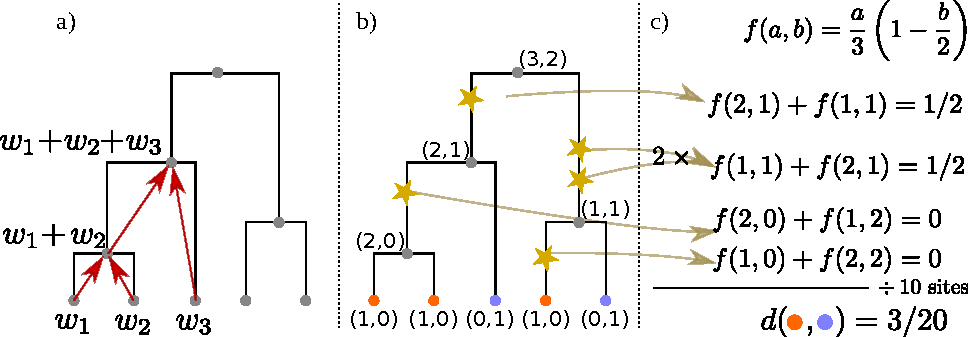
\includegraphics{figures/divergence_diagram}
    \caption{
        An example of computing sequence divergence between red nodes and blue nodes
        from seven mutations at distinct sites in a sequence of length 10 using the tree.
        The summary function, $f(a,b) = (a/3)(1-b/2)$ gives the probability that
        an allele found in $a$ of the red nodes and $b$ of the blue nodes is present in
        a randomly chosen red node but not in a randomly chosen blue node.
        \textbf{(a)} Weights are assigned to each subtree by adding together the weights of any children,
        plus the weight of the node itself, if it is a sample.
        \textbf{(b)} In this example, subtree weights $(a,b)$ record how many red nodes ($a$)
        and how many blue nodes ($b$) lie in that subtree.
        \textbf{(c)} The summary function shown is applied to both the weight below 
        and the weight not below each mutation,
        so for instance the mutation above the node with weights $(2,1)$
        contributes $f(2,1) + f(1,1) = 1/3 + 1/6 = 1/2$.
        The final value for divergence is the sum of these values divided by 10,
        the total number of sites.
        \label{fig:divergence_diagram}
    }
\end{figure}


%%%%%%%%%%%%%%%%%%
\subsection*{Tree sequences}

Before defining the different classes of statistic,
it will help to establish a little more notation.
A tree sequence efficiently describes how a set of $n$ sampled chromosomes
are related to each other along a (linear) genome of length $L$ \citep{kelleher2016efficient,kelleher2018efficient}.
% These trees are highly correlated,
% a fact which allows them to be stored and processed very efficiently,
% as described in \citet{kelleher2018efficient}.
From the tree sequence can be extracted a sequence of trees,
$\treeseq = (T_1, T_2, \ldots, T_{n(\treeseq)})$
and a sequence of breakpoints $0 = a_0 < a_1 < \cdots < a_{n(T)} = L$,
where $T_k$ describes the genealogical relationships of the samples
over the segment of genome betwen $a_{k-1}$ (inclusive) and $a_k$ (exclusive).
We say that tree $T_k$ \emph{covers} the (half-open) segment $[a_{k-1}, a_k)$,
and call the length of this segment its \emph{span}, denoted $L_k = a_k - a_{k-1}$.
We refer to the branches in each tree using the most recent node,
so for instance the branch describing a relationship where $u$ is the child of $v$
is associated with $u$.
The \emph{length} of this branch is the difference in birth times of $v$ and $u$,
and is denoted $t_T(u)$ (dropping $T$ if it is clear from context).
Note that although the same parent-child relationship may exist across many adjacent trees
(this is called an ``edge''),
rearrangements of genealogical relationships
can cause the precise set of samples that lie below that edge to differ across
trees.


%%%%%%%%%%%%%%%%%%
\subsection*{Node statistics}

Perhaps the most natural way to summarise weights on the tree
is simply to examine the values at each node.
This would allow us, for instance, to 
count the number of samples that inherit from each node in the tree. 
Averaged across trees,
this tells us what proportion of the sample's genomes were inherited from each node.
Motivated by this, we define the
\textbf{node statistic} for node $u$
associated with summary function $f()$ and sample weights $\iw$
to be the sum of $f()$ applied to the weight of the subtree below node $u$
and to the remaining weight,
averaged across the genome:
\begin{align}
    \node(f, \iw)_u
    =
    \frac{1}{L} \sum_{k=1}^{n(\treeseq)} L_k \left( f(\nw_{T_k}(u)) + f(\tiw - \nw_{T_k}(u)) \right).
\end{align}
The weight $\nw_{T_k}(u)$ is the subtree weight below $u$ in the tree $T_k$,
and $\tiw - \nw_{T_k}(u)$ is the sum of all weights \emph{not} in the subtree below $u$ in $T_k$.
% i.e., the length of the segment of genome that the tree extends for.
% If this is computed over only a ``window'' of the genome
% then $L_k$ is replaced by the length of the portion of that window
% that $T$ extends for.

\paragraph{Polarisation}
In this definition we have associated with each node the summary of both the weight below the node
\emph{and} the weight not below the node.
Would it not be more natural to only include the first term, $f(\nw_{T_k}(u))$?
The reason for this definition is that it does not depend on the location of the root of the tree,
which in practice may be unknown.
Statistics of genotype sequence defined below in an analogous way
will not depend on knowledge of which allele is ancestral, i.e., on \emph{polarisation} of alleles.
For this reason, the node statistic above is the \emph{unpolarised} version,
while a \emph{polarised} node statistic is defined without the second term:
\begin{align}
    \text{(polarised)} \qquad
    \nodep(f, \iw)_u
    =
    \frac{1}{L} \sum_{k=1}^{n(\treeseq)} L_k f(\nw_{T_k}(u)) .
\end{align}

We will use weights that count number of samples below each node
sufficiently often that we give them a special name --
for a subset set $S$ of samples,
the \emph{indicator weights of $S$} are the sample weights $\bone_S$ with
$\bone_S(u) = 1$ if $u \in S$ and $\bone_S(u) = 0$ otherwise.

\begin{example}[Ancestry proportions] \label{ex:ancestry_props}
    If $\iw$ are the indicator weights of the set $S$ of $n$ samples,
    and then $\iw_u / n$ is the proportion of the samples in $S$ that lie below $u$.
    Therefore, if $f(x) = x / n$,
    then $\nodep(f, \iw)_u$ is the proportion of the genomes of $S$
    that are inherited from (ancestor) $u$.
\end{example}

Node statistics only make sense in the context of the tree sequence,
but provide a useful bridge to the next type of statistic,
which are defined directly in terms of the genotypes.


%%%%%%%%%%%%%%%%%%
\subsection*{Site statistics}

Now we arrive at our primary goal, which is to compute statistics from \emph{genomes}
using this framework.
To do this, we assume that the genetic variation data is embedded in a tree sequence,
but the trees are used only for efficiency --
the results will not depend on the trees in any way
(with the only exception being if the ancestral allele is assumed to be known, as discussed below).

The summaries we defined above for each node in each tree
extend nicely to genetic variants 
-- just as a node weight contains information about which samples are below the node and which are not,
so we can summarise patterns of genetic variation by summing up weights of all samples
that carry a given allele.
So, we define \emph{allele weights} to be
the total weight of all sample nodes who have inherited that allele.

\begin{definition}[Allele weights]
    The \emph{allele weight} for allele $a$ at site $j$ is the sum of the weights
    of all sample nodes inheriting this allele:
    \begin{align*}
        \aw_j(a) = \sum_{v \st g_j(v) = a} \iw(v) ,
    \end{align*}
    where the sum is over all sample nodes $v$ for which
    $g_j(v)$, the allele carried by node $v$ at site $j$, is equal to $a$.
\end{definition}

If there has been only one mutation at the site,
then $\aw_j(a)$ is equal to the weight of the subtree below the mutation that produced $a$.
More generally, $\aw$ is not necessarily equal to a subtree weight
but is easily computable from them.

Using allele weights,
we define the \textbf{site statistic} of site $j$ computed using a summary function $f()$
and a set of sample weights $\iw$
to be the sum of $f()$ applied to each of the allele weights:
\begin{align}
    \site(f, \iw)_j
    &=
    \sum_{a} f(\aw_j(a)) ,
\end{align}
where the sum is over all unique alleles at site $j$.

Of course, we often want to summarize statistics across regions of the genome (``windows'').
To do this, we overload notation somewhat and use a subscript $[i,j)$ to denote an average
over the corresponding portion of the genome:
\begin{align}
    \site(f, \iw)_{[i,j)}
    &=
    \frac{1}{j-i} \sum_{k=i}^{j-1} \site(f, \iw)_k
\end{align}
Since we have required $f(0) = f(\tiw) = 0$,
the sum will only be affected by polymorphic sites,
although the normalization is always by total number of sites, to allow comparison between regions.


In the definition above we simply sum over all alleles at each site.
However, sometimes it is useful to distinguish the \emph{ancestral} allele
(i.e., the allele at the root of the tree) from the remaining derived alleles.
This allows statistics in principle to differentiate ancestral from derived alleles,
information which is available in practice (albeit noisily),
and one way to make use of this information is to sum over only derived alleles.
Analogously to the above,
we say a site statistic is \textbf{polarised} if we do this,
defining
\begin{align} \label{eqn:site_polarised}
    \text{(polarised)} \qquad
    \sitep(f, \iw)_j
    &=
    \sum_{a \in D_j} f(\aw_j(a)) ,
\end{align}
where $D_j$ denotes the set of all alleles at site $j$ except the allele at the root of the tree.
Note that this may not be quite what is expected,
for instance, if there has been a back mutation to the ancestral allele at some point in the tree,
or if there have been mutations to distinct alleles on different parts of the tree
such that the ancestral allele is no longer present.
However, since these situations depend on multiple mutations occurring at a single site,
they are relatively rare in practice.

Now we have defined a general, abstract, framework.
Is it good for anything?
Next we give some examples.

\begin{example}[Nucleotide diversity] \label{ex:site_diversity}
    Suppose we want to compute the mean density of nucleotide differences
    in a group $S$ of $n$ sequences.
    To do this,
    % let $\iw_u = 1$ for $u \in S$ and $\iw_v = 0$ otherwise,
    let $\iw = \bone_S$,
    so that $\nw(u)$ gives the number of nodes in $S$ below $u$,
    and define
    \begin{align*}
        f(x) = \frac{x (n - x)}{n (n-1)} .
    \end{align*}
    Then $\site(f, \iw)_{[a,b)}$ is mean nucleotide diversity in the region between $a$ and $b$.
\end{example}

\begin{example}[Nucleotide divergence] \label{ex:site_divergence}
    Now suppose we want to compute the mean density of nucleotide differences
    \emph{between} two nonoverlapping groups of samples, $S_1$ and $S_2$,
    with $n_1$ and $n_2$ samples, respectively.
    As before,
    let $\iw_j = \bone_{S_j}$,
    so that $\nw_{j}(u)$ gives the number of nodes in $S_j$ below $u$.
    Then we define
    \begin{align*}
        f(x_1, x_2) = \frac{x_1 (n_2 - x_2)}{n_1 n_2} .
    \end{align*}
    Then $\site(f, \iw)_{[a,b)}$ is mean nucleotide divergence between the two groups
    in the region between $a$ and $b$.
\end{example}

\begin{example}[Segregating sites] \label{ex:segregating_sites}
    Again, let $\iw = \bone_{S}$ for a group of $n$ sequences,
    and now define
    \begin{align*}
        f(x) = \begin{cases}
            1 - \frac{x}{n} \qquad &\text{if } x > 0 \\
            0 \qquad &\text{otherwise} .
        \end{cases}
    \end{align*}
    In computing $\site(f, \iw)_{[a,b)}$, the function $f()$ is given the number of samples in $S$
    that inherit each allele.
    A site with $k$ distinct alleles that segregate in $S$ with proportions $p_1 + \cdots + p_k = 1$
    contributes $f(p_1) + \cdots + f(p_k) = (1 - p_1) + \cdots + (1 - p_k) = k - 1$ to the statistic.
    Therefore, $\site(f, \iw)_{[a,b)}$, is the minimum number of derived mutations per unit length,
    which is the density of segregating sites if all sites are biallelic.
\end{example}

\begin{example}[Phenotypic correlations] \label{ex:site_correlations}
    Suppose that for each sample $u$ we have a numeric phenotype, denoted $z(u)$,
    and we want to compute the correlation between this phenotype
    and the genotype at each site in the tree sequence.
    For convenience, suppose $z$ is normalized 
    % so that $\sum_u z(u) = 0$ and $\sum_u z(u)^2/(n-1) = 1$.
    to have mean zero and variance 1.
    Then, if $g_j$ is a vector of binary genotypes (so $g_j(u) = 1$ if $u$ carries the derived allele),
    then the covariance of $z$ with $g_j$ is just $\sum_u z(u) g_j(u) = \sum_{u \st g_j(u) = 1} z(u)$,
    i.e., the sum of the phenotypes of all samples carrying the derived allele,
    divided by $(n - 1)$, where $n$ is the number of samples.
    Since the phenotypes sum to zero, this is also equal to 
    $- \sum_{u \st g_j(u) = 0} z(u)$.
    If $p_j = \sum_u g_j(u)$ is the derived allele frequency at site $j$,
    then the variance of $g_j$ is $n p_j (1-p_j) / (n-1)$,
    and so the squared correlation can be calculated as a sum across the two alleles:
    \begin{align*}
        r_j^2 =
        \frac{\left( \sum_{u \st g_j(u) = 0} z(u)\right)^2}{2p(1-p)n(n-1)} 
        + \frac{\left( \sum_{u \st g_j(u) = 1} z(u)\right)^2}{2p(1-p)n(n-1)}  .
    \end{align*}
    We can compute this as a site statistic by defining $\iw_{1}(u) = z(u)$, and $\iw_{2}(u) = 1/n$,
    and $f(x_1, x_2) = x_1^2 / (2 x_2 (1 - x_2) n (n-1))$:
    then $\site(\iw, f)_j = r_j^2$ is the squared correlation between $z$ and the allele at site $j$.
\end{example}

%% Check that math:
% n <- 10; z <- rnorm(10); z <- (z - mean(z))/sd(z); g <- rbinom(n, size=1, prob=1/2); p <- mean(g)
% c(cov(z,g), sum(z*g)/(n-1))
% c(cor(g,z), sum(g*z)/sqrt(n*(n-1)*p*(1-p)))

\begin{example}[Patterson's $f_4$] \label{ex:site_f4}
    Given four disjoint groups of samples, $S_1$, $S_2$, $S_3$, and $S_4$,
    Patterson's $f_4(S_1, S_2; S_3, S_4)$ statistic for an allele with frequency $p_i$ in group $S_i$
    is $(p_1 - p_2)(p_3 - p_4)$ (and then this is typically averaged over sites).
    To rewrite this as a sum over alleles, note that
    $p_1 - p_2 = p_1 (1 - p_2) - (1 - p_1) p_2$,
    and so the statistic counts with positive weight
    alleles that split $S_1$ and $S_3$ from $S_2$ and $S_4$,
    and negative weight ones that split $S_1$ and $S_4$ from $S_2$ and $S_3$.
    Therefore, if as before we
    let $\iw_j = \bone_{S_j}$
    % let $\iw_{ju} = 1$ if $u \in S_j$
    (so that $\iw_{ju}$ tells us the number of samples in $S_j$ descended from $u$),
    and write $n_i$ for the number of samples in $S_i$, and
    \begin{align*}
        f(x_1, x_2, x_3, x_4)
        =
        \frac{x_1}{n_1}
        \frac{x_3}{n_3}
        \left(1 - \frac{x_2}{n_2}\right)
        \left(1 - \frac{x_4}{n_4}\right)
        -
        \left(1 - \frac{x_1}{n_1}\right)
        \left(1 - \frac{x_4}{n_4}\right)
        \frac{x_2}{n_2}
        \frac{x_3}{n_3} ,
    \end{align*}
    then $\site(\iw, f)_{[a,b)}$ is equal to Patterson's $f_4(S_1, S_2; S_3, S_4)$ statistic
    for the region of the genome between $a$ and $b$.
\end{example}

\paragraph{Polyallelic sites}
The statistics defined above map exactly onto those standard in population genetics
when all sites are biallelic.
There is not a consensus in the field
on how to use sites with more than two alleles, but the most common practice is
to reduce to biallelic data, by either discarding other sites
or by marking all non-ancestral alleles as (the same) ``derived'' allele.
We choose to define statistics in a way that still makes formal sense for polyallelic sites,
so that for instance a site with ancestral allele $A$ and derived alleles $C$ and $T$
would have site statistic $f(\aw(A)) + f(\aw(C)) + f(\aw(T))$.
This is a natural defintion in that it agrees with what is obtained by
looking at pairwise haplotype differences.
For instance, the definition of nucleotide divergence in Example \ref{ex:site_divergence}
gives the probability that a randomly chosen sample from each set differ.
This definition makes sense even at polyallelic sites,
and (as we discuss below) has a natural correspondence to statistics related to branch lengths.


%%%%%%%%%%%%%%%%%%
\subsection*{Branch statistics}

Genetic variation is informative about many processes
precisely because it tells us about the underlying patterns of genealogical relatedness.
In other words, the genomes are useful in so far as they tell us about the trees.
In the case where we actually have the trees, or a good proxy for them,
it is natural to summarize them directly, rather than working indirectly with the genotypes.
If we assume that no two mutations occur at the same genomic position --
i.e., the \emph{infinite sites model} --
then there is a natural correspondence between summaries of genotypes and summaries of tree shape.
If mutations occur at a constant rate in time and along the genome,
then the \emph{expected} number of mutations that occur somewhere along a branch of a tree
over some segment of genome
is equal to the mutation rate multiplied by the length of the segment and by the length of the branch.
In other words, the ``area'' of a branch in a tree of the tree sequence,
defined as its span (right minus left endpoint) multiplied by its length (parent time minus child time)
and scaled by the mutation rate,
is equal to the expected number of mutations that will land on it.
If the mutation rate is constant,
then this gives us an isometry --
measuring tree distances in branch lengths versus in numbers of mutations
are equal in expectation, up to a constant.

This makes it natural to define
a statistic of tree shape by summing these expected contributions across its branches.
We define the \textbf{branch statistic} of a single tree $T$ with span $L$
obtained from summary function $f()$
and sample weights $\iw$ with total weight $\tiw = \sum_u \iw(u)$
to be the sum of the area of each branch in each tree
multiplied by the summary function applied to its subtree weight:
\begin{align}
    \branch(f, \iw)_T
    &=
    \frac{1}{L} \sum_{u \in T} t_{u} \left( f(\nw_{T}(u)) + f(\tiw - \nw_{T}(u)) \right)  ,
\end{align}
where $t_{u}$ is the length of the branch above node $u$ in tree $T$
and $\nw_{T}(u)$ is the total weight of the subtree of $T$ below $u$ (as defined above).
The term $\tiw - \nw_{T}(u)$ gives the total weight \emph{not} in the subtree of $T$ below $u$,
because the sum of all weights in the tree is always $\tiw$.
The value $f(\nw(u))$ is the summary value that would be added to a site statistic
if a single mutation occurred on the branch above $u$,
and $f(\tiw - \nw_{T}(u))$ is the value that would be added due to its complementary allele,
so $\branch(f, \iw)_T$ gives the expected contribution of this branch to $\site(f, \iw)$,
per unit of sequence length that the tree $T$ covers.

An example is shown in Figure~\ref{fig:branch_site_diagram},
showing how the $f_4$ site statistic assigns a weight to each mutation
depending on the frequencies in each of the four sample sets below it,
and how the corresponding branch statistic assigns the same weight to those branches.

\begin{figure}
    \centering
    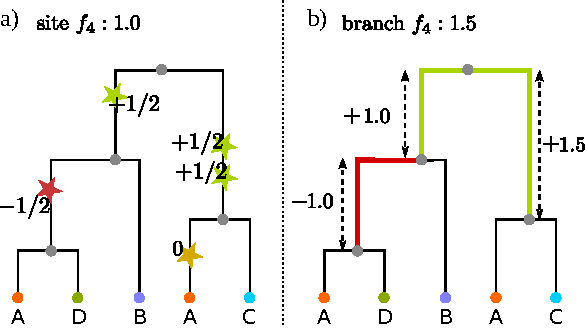
\includegraphics{figures/branch_site_diagram}
    \caption{
    Computing the $f_4(A,B;C,D)$ statistic on a tree.
    \textbf{(a)} Each mutation is given weight equal to $(p_A - p_B)(p_C - p_D)$,
    where $p_X$ is the proportion of the samples inheriting that mutation in set $X$
    (shown in labels at the bottom).
    Note that each of the mutations shown occurs at a distinct site, so there is no backmutation.
    \textbf{(b)} Each branch is assigned weight equal to the weight that would be assigned
    to any mutation falling in it, and then the branch $f_4$ statistic
    is the sum over these weights, multiplied by the length of the branch
    (and the span of the tree, not depicted).
        \label{fig:branch_site_diagram}
    }
\end{figure}


This defines a statistic for a single window,
but in practice it is probably most useful to average branch statistics
over a region of the genome,
which we do by averaging the tree statistics over the region
with probabilities proportional to the trees' spans.
We write this with similar notation:
\begin{align}
    \branch(f, \iw)_{[c,d)}
    &=
    \frac{1}{d-c} \sum_{k=1}^{n(\treeseq)} \ell_k(c,d) \branch(f, \iw)_{T_k} ,
\end{align}
where $\ell_k(c,d)$ is the length of the region in $[c,d)$ that the tree $T_k$ extends for
(i.e., $T$ covers the half-open interval $[a_{k-1},a_k)$,
so $\ell_k(c,d) = \max(0, \min(d,a_k) - \max(c,a_{k-1}))$).

The \emph{polarised} version of this statistic
is defined analogously to the Node and Site versions:
\begin{align} \label{eqn:branch_polarised}
    \text{(polarised)} \qquad
    \branchp(f, \iw)_T
    &=
    \sum_{u \in T} f(\nw_{T}(u)) ,
\end{align}
and $\branchp(f, \iw)_{[c,d)}$ is defined using $\branchp(f, \iw)_T$ as before.
However, the correspondence between the polarised statistics is less tight
than for the unpolarised ones.


\begin{example}[Mean TMRCA] \label{ex:branch_diversity}
    If we take $\iw$ and $f$ exactly as in the ``Nucleotide diversity'' example above,
    then $f(u)$ gives the probability that the branch above $u$
    lies on the path from two randomly chosen samples from $S$
    on the path up to their most recent common ancestor (MRCA).
    Therefore, $\branch(f, \iw)$ for these choices
    gives the mean total distance in the tree between two samples from $S$,
    averaged across the sequence.
    This is twice the mean TMRCA if the samples are all from the same time.
\end{example}

\begin{example}[Phenotypic correlation with pedigree] \label{ex:branch_correlation}
    If we take $\iw$ and $f$ as in the ``Phenotypic correlations'' example above,
    what does $\branch(f, \iw)$ tell us?
    The statistic tells us the \emph{expected} correlation between phenotype and any mutations
    appearing on the tree, which is a summary of how much local relatedness
    aligns with similarity in phenotype.
\end{example}


\begin{example}[Patterson's $f_4$] \label{ex:branch_f4}
    Suppose that the four subsets each consist of only a single sample.
    The summary function $f(x_1, x_2, x_3, x_4)$ for the $f_4$ statistic
    then assigns weight 1 to any branch that separates $x_1$ and $x_3$ from $x_2$ and $x_4$,
    and weight -1 to any branch that separates $x_1$ and $x_4$ from $x_2$ and $x_3$.
    The statistic $\branch(f, \iw)$ therefore
    gives the difference in averages of these two types of branch,
    averaged over choices of samples from the sample sets and averaged across the genome.
\end{example}

%%%%%%%%%%%%%%%%%%
\section*{Duality of site and branch statistics}

Under a neutral, infinite-sites model of mutation with constant mutation rate across time,
the expected number of mutations per branch is proportional to its length.
This implies an isormorphism between ``site'' and ``branch'' statistics defined above,
which is discussed in more detail in \citet{ralph2019empirical}.
For instance, the site statistic of Example \ref{ex:site_diversity} (genetic diversity)
and the branch statistic of Example \ref{ex:branch_diversity} (mean TMRCA)
use the same summary function $f(x) = x(n-x)/n(n-1)$.
These are closely related because under an infinite-sites model of mutation,
two sequences differ at a site only if there has been a mutation somewhere on the branches going back
to their most recent common ancestor,
and so if mutations occur with constant rate,
the expected value of genetic diversity,
averaging over mutational noise give the tree sequence,
is equal to the mutation rate multiplied by the average distance between the two in the trees.

This relationship is true more generally.
In fact, for any region of the genome between $a$ and $b$,
with $\treeseq_{[a,b)}$ the trees spanning that interval,
\begin{align}
    \branch(f, \iw)_{[a,b)}
    =
    \E\left[ \site(f, \iw)_{[a,b)} \given \treeseq_{[a,b)} \right] ,
\end{align}
where the expected value averages over infinite-sites mutations with rate 1
(and so lengths are measured in units of expected numbers of mutations).
Let's unpack this statement a bit more: what exactly is the mutational model?
First, we are taking the mutation rate to be 1, i.e.,
the expected number of mutations that occur on a region of the genome of length $\ell$
over $t$ units of time is equal to $\ell t$.
This just amounts to a change of units --
for instance, if genome length is measured in nucleotides,
and the probability of mutation is $\mu$ per nucleotide and per generation,
then we are measuring times in units of $1/\mu$ generations.
Second, we are assuming that the probability of per-site mutation is low enough
that no two mutations occur at the same site
-- the fact that they do, occasionally, means that this is an approximation.
Third, we are assuming that mutation rates are constant through time and across the genome.
Of course, the statement remains true if we can measure distance along the genome and time
in a way that mutation rates are constant, but how these vary is generally unknown.

Note that the expected product of two site statistics,
$\E[\site(f, \iw) \site(g, \iw')]$
is not equal to the product of the two branch statistics, $\branch(f, \iw) \branch(g, \iw')$,
because they are not independent.
However, it is always possible to define a branch statistic that
gives the expected value of the product.
How to do this is described in \citet{ralph2019empirical}.

In this view,
site statistics are noisy approximations to the corresponding branch statistic
-- but, how noisy?
How big is the contribution of mutation to the overall sampling variance of a statistic?
Concretely the law of total variance lets us partition the variance of a site statistic
into the contributions of mutation and demographic noise:
\begin{align*}
    \var[\site(f, \iw)_{[a,b)}] 
    &=
        \E\left[ \var\left[\site(f, \iw)_{[a,b)} \given \treeseq_{[a,b)}\right] \right] 
        + \var\left[ \E\left[\site(f, \iw)_{[a,b)} \given \treeseq_{[a,b)}\right] \right] \\
    &=
        \E\left[ \var\left[\site(f, \iw)_{[a,b)} \given \treeseq_{[a,b)}\right] \right] 
        + \var\left[ \branch(f, \iw)_{[a,b)} \right] .
\end{align*}
The first term, the variance of the statistic given the trees,
is the contribution to variance of mutation,
while the second term, the variance of the branch statistic,
is the contribution of demographic variation, including drift.


%%%%%%%%%%%%%%%%%%%%%%%%%%%%%%%%%%%%%%%%
\subsection*{Branch statistics for population genetics}

We examined the contributions of mutation and demography to noise
in two simulations where population genetic (site) statistics
are important in making inferences:
detecting recent selective sweeps,
and detecting introgression.

Figure~\ref{fig:sweep_duality} shows windowed
diversity along the chromosome following a few selective sweeps.
The top two plots compare ``branch'' diversity -- i.e., as computed only with tree shape --
to ``site'' diversity computed from sequence generated by 20 independent assignments of mutations to the same tree sequence,
with mutation rates $10^{-9}$ and $10^{-8}$, respectively.
We see that as the mutation rate increases, the signal of decrease in diversity around swept loci becomes more clear,
and approaches ``branch'' diversity.
These were computed using the entire population of 1,000 individuals;
how does sampling variance contribute?
Not much, it turns out -- the bottom plot shows both site and branch diversity
computed from 20 nonoverlapping groups of 100 samples.
Neither site or branch diversity vary much between these samples,
implying that the subsample gives us a good estimate of the whole-population values of each.
However, as we see in the top figure,
whole-population site diversity is itself only a quite noisy estimator of branch diversity.
The same things are shown in Supplementary Figure \ref{sfig:sweep_duality_10K}
for a simulation with 10,000 individuals, which shows similar patterns.
Only the last of these plots is possible to directly observe in real data:
in the top two plots,
the spread of independent replicates of mutational noise (black lines)
about their expectation based on the tree sequence (red line)
is unobservable, although estimable.


\begin{figure}
    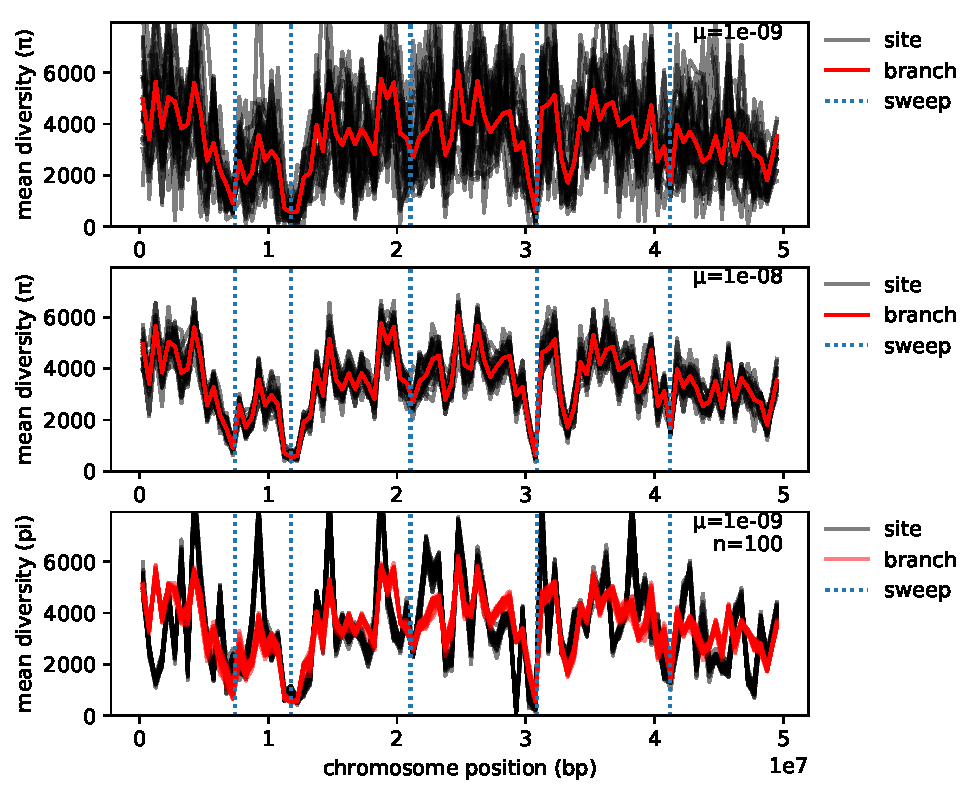
\includegraphics{{figures/swept.1000.999.1e-09.diversity}.pdf}
    \caption{
        Mean genetic diversity and time to most recent common ancestor
        in 500Kb windows along a 50Mb genome (0.5 Morgans) following several selective sweeps.
        In each case, ``site'' is mean genetic diversity (Tajima's $\pi$) divided by mutation rate,
        and ``branch'' is the corresponding branch statistic described above.
        The tree sequence was produced by simulating mutations under positive selection with mutation rate $10^{-12}$ 
        in a population of size 1000 for 400 generations using SLiM,
        followed by recapitation with $N_e=1000$.
        The selected alleles at the marked sites have selection coefficients between 0.08 and 0.25,
        and are at frequencies 96.8\%, 100\%, 16.25\%, 100\%, and 82.6\% in the final generation, respectively.
        All curves use the same tree sequence, including selected mutations,
        and with additional neutral mutations added.
        \textbf{(top)}
        Diversity within the entire population,
        computed using for mode ``site'' from 20 independent assignments of mutations to the same tree sequence with mutation rate $\mu = 10^{-9}$.
        \textbf{(middle)}
        As in the top panel, but with mutation rate $\mu=10^{-8}$,
        showing that as mutation rate increases, mode ``site'' (divided by $\mu$) converges to mode ``branch''.
        \textbf{(bottom)}
        ``Site'' and ``branch'' diversity within 20 disjoint samples of size 100 each,
        computed on a single tree sequence with mutation rate $\mu = 10^{-9}$.
        \label{fig:sweep_duality}
    }
\end{figure}


As another example, we simulated an ``admixture'' scenario:
a first population of size $N=1000$ splits into two of equal size,
then after $N$ generations, the second population splits,
after another $N$ generations, the third population splits again,
and for the final $N$ generations populations 2 and 3
have per-capita migration rates of $4/N$ to each other.
In this situation, a significantly negative $f_4(1,2;3,4)$ is expected,
which we indeed find, with a mean value of around -700.
Using various sample sizes, mutation rates, and window sizes, we then
calculated this $f_4$ statistic in windows along a 100Mb genome,
and show the standard deviation of both ``site'' and ``branch'' statistics across windows
in Figure \ref{fig:introf4}.
Since the genome is uniform (no selection or variation in recombination or mutation),
this standard deviation is a measure of noisiness.
As expected, site statistics are noisier than branch statistics,
by a factor that depends mostly on the ratio of mutation to recombination rates.
The results suggest that branch statistics would provide substantially better resolution
at small scales along the genome, especially if mutation rate is lower than recombination rate.
However, in practice imperfect estimation of the tree sequence
would introduce additional noise,
so it remains to be seen if the improvement could be made in practice.

\begin{figure}
    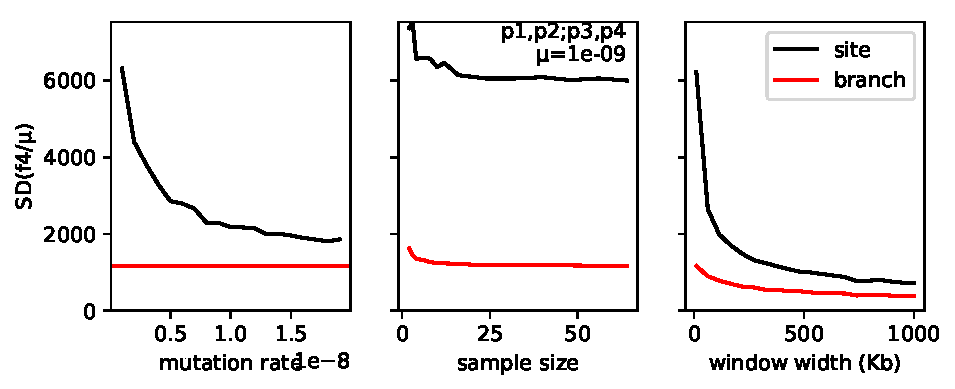
\includegraphics{{figures/intro/introgressed.1000.23.10000.1e-09.f4sd}.pdf}
    \caption{
        Standard deviation of site (black) and branch (red) $f_4(1,2;3,4)$
        in windows along a 100Mb genome, as a function of
        \textbf{(left)} mutation rate,
        \textbf{(middle)} sample size, and
        \textbf{(right)} window width.
        The recombination rate $10^{-8}$,
        and unless otherwise stated, the mutation rate was $10^{-9}$,
        the window width was 10Kb,
        and the entire population (1000 diploids in each of four populations) were used.
        \label{fig:introf4}
    }
\end{figure}


%%%%%%%%%%%%%%%%%%
\section*{Application to 1000 Genomes tree sequences}

We do not know the true genealogies underlying real data,
but recent methods are available to estimate them.
To evaluate the correspondence between site and branch statistics
in real data,
we calculated mean sequence diversity along chromosome 20 from the 1000 Genomes dataset
in 1Mb windows separately in each of the five continental groupings,
calculated using the site statistic described in Example~\ref{ex:site_diversity},
and compared this to the corresponding branch statistic (of Example~\ref{ex:branch_diversity})
as calculated from three inferred tree sequences:
by tsinfer \citep{tsinfer}, which does not attenpt to estimate well-calibrated node times,
(2) by GEVA \citep{geva}, which aims to calibrate the node times reported by tsinfer,
and (3) by Relate \citep{relate}, an independently developed method.
All calculations were done only using the portions of the chromosome
passing the ``strict'' mask for sequencing accessibility.
Separate curves for each of the 26 populations are shown in Supplemental Figure \ref{fig:chr20_full}.

The comparisons are shown in Figure~\ref{fig:chr20}.
Of these methods, branch diversity from tsinfer shows the worst agreement with site diversity,
which is unsurprising as tsinfer makes no attempt to provide well-calibrated node times,
and only aims to provide consistent tree topologies.
The two methods that infer node times differ substantially,
with Relate showing a significantly tighter agreement than GEVA.
Does this mean that Relate is doing a better job at inferring the tree sequence than GEVA?
This is highly suggestive, but not entirely clear.

\begin{figure}
    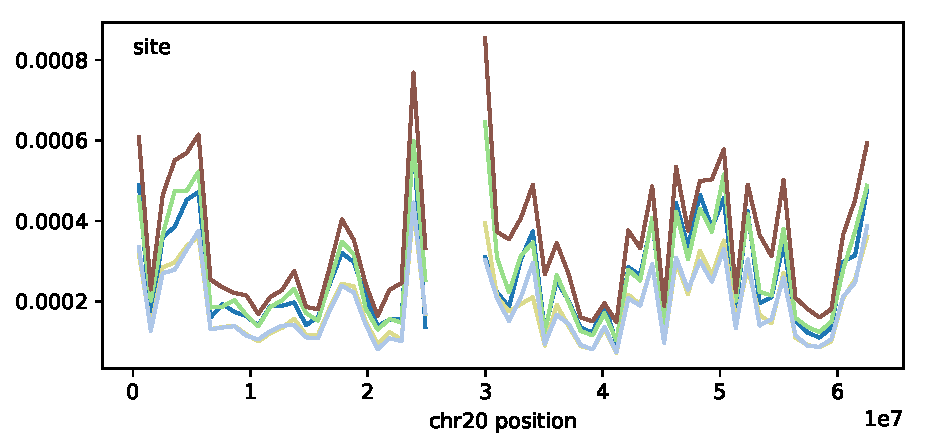
\includegraphics[width=0.5\textwidth]{{figures/1kg/relate_chr20.site.1000000.region.diversity}.pdf}
    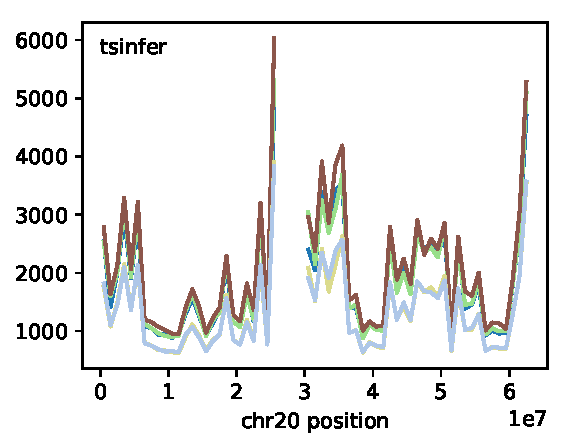
\includegraphics[width=0.5\textwidth]{{figures/1kg/1kg_chr20.branch.1000000.region.diversity}.pdf}
    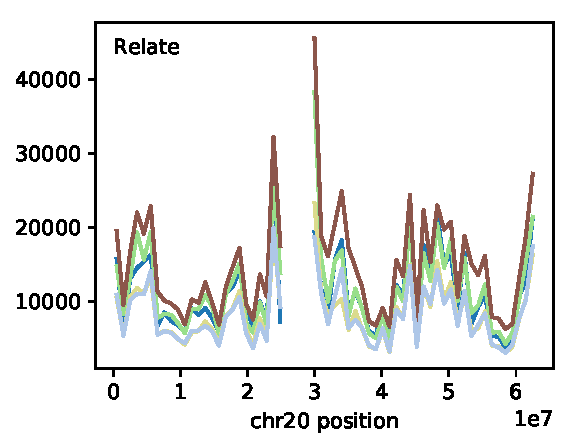
\includegraphics[width=0.5\textwidth]{{figures/1kg/relate_chr20.branch.1000000.region.diversity}.pdf}
    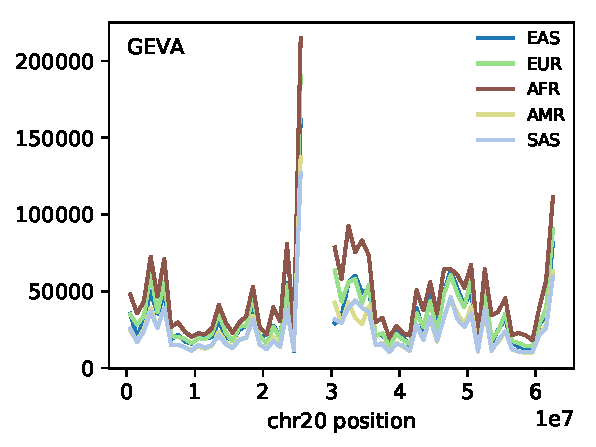
\includegraphics[width=0.5\textwidth]{{figures/1kg/tgp_geva_chr20.branch.1000000.region.diversity}.pdf}
    \caption{
        \textbf{(top left)} Mean sequence diversity 
        in 1Mb windows along human chromosome 20 of the 1000 Genomes Project,
        and the dual branch statistic as calculated from tree sequences inferred by
        \textbf{(top right)} tsinfer,
        \textbf{(bottom left)} Relate, and
        \textbf{(bottom right)} GEVA.
        \label{fig:chr20}
    }
\end{figure}

In practice, we do not expect branch and site diversity to agree exactly,
because of local differences in mutation rate and intensities of selected mutations.
For instance, regions in which a high proportion of potential mutations are deleterious
are expected to have a diversity for two reasons:
first, the deleterious mutations themselves are less likely to be found,
and second, the indirect effect of deleterious mutations on nearby sites reduces typical tree height
and thus diversity at even neutral, linked sites \citep{background_selection}.
The first effect would cause site and branch statistics to differ,
because it effectively reduces the mutation rate in the region
and violates the assumption of independence of mutations given the trees.
However, the second effect does not affect the correspondence between site and branch statistics,
since it is mediated by tree shape.
However, it is generally unknown how much mutation rate varies along the genome
\citep[but see][]{mut_rate_varies}
or how dense are targets of selection \citep{how_important_is_selection}.
For this reason, it is very interesting to see how close a correspondence between site and branch
statistics it is \emph{possible} to obtain --
it is tempting to say that the best tree sequence would obtain
as tight a match between site and branch statistics as possible,
with remaining variation explained by selection and/or mutation rate variation.


%%%%%%%%%%%%%%%%%%%%%
\subsection*{Time stratification of statistics}

Thus far we have examined how statistics vary along the genome.
A tree sequence allows us access to another dimension: time.
Next, we use node statistics to display the \emph{time} distribution of admixture signal
in the tree sequences inferred by tsinfer/GEVA and by Relate.
The ``node'' $f_4(A, B; C, D)$ statistic for four populations $A$, $B$, $C$, and $D$
can be used to calculate, for each node, the average of $(p_A - p_B)(p_C - p_D)$
across the portion of the genome that the node is present in the tree sequence,
where $p_A$ is the proportion of samples in $A$ that lie below that node, etcetera.
A node with a large value will contribute a large amount to the site or branch $f_4$.


\begin{figure}
    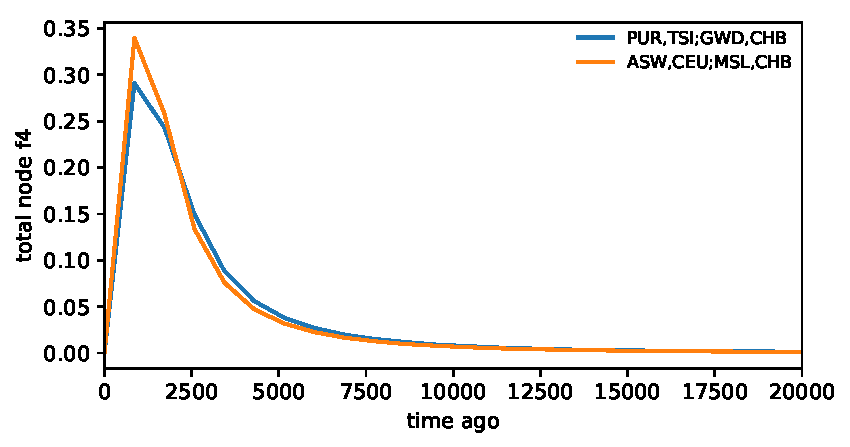
\includegraphics{{figures/1kg/relate_chr20.node.f4}.pdf}
    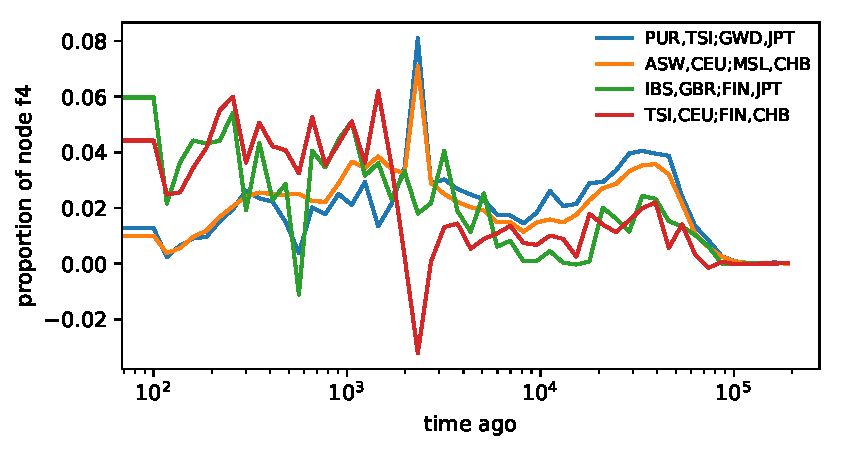
\includegraphics{{figures/1kg/tgp_geva_chr20.node.f4}.pdf}
    \caption{
        Time distribution of signal for two $f_4$ statistics
        in tree sequences inferred by \textbf{(top)} Relate and \textbf{(bottom)} GEVA.
        Both 
        \label{fig:node_f4}
    }
\end{figure}



%%%%%%%%%%%%%%%%%%
\section*{Efficient algorithms and implementation}

%%%%%%%%%%%%%%%%%%%%%
\subsection*{Algorithms}
write-up of algorithm for maintaining branch statistic across trees

%%%%%%%%%%%%%%%%%%%%%
\subsection*{Speed}

compare speed to scikit-allel






%%%%%%%%%%%%%%%%%%%%%%%
\section*{Discussion}

In this paper,
we consider only so-called \emph{single site} statistics
(which we will define concretely shortly).
Extensions to statistics involving the pairwise joint distribution of genotypes across sites,
such as linkage disequlibrium,
are straightforward, and are planned for future work.
Haplotype-based statistics may require a different class of algorithms.


\paragraph{Diploid statistics}
The statistics we develop here are in essence \emph{haploid} statistics.
These tools can be used to compute a statistic about polyploid individuals,
but they do not scale to large numbers of individuals.
For instance, to compute the heterozygosity of a set of samples
-- this is $(1/N) \sum_{i=1}^N 2 p_i (1-p_i)$, where $p_i$ is the derived allele frequency
in the $i^\text{th}$ individual --
one would need to have an entry in the weight vector for \emph{each individual}.
The genotype of a diploid at a site with a single mutation that occurred on the branch above node $n$
is determined by where that node falls relative to the diploid's two haplotypes in the tree:
if $n$ is on the path from either haplotype to their MRCA, the individual is heterozygous;
if $n$ is on the path from the MRCA to the root, the individual is homozygous derived;
and the individual is homozygous ancestral otherwise.
This suggests the following generalization of our current scheme for diploids:
for a list $(I_1, \ldots, I_N)$ of pairs of nodes,
and two vectors $w^{(1)}$ and $w^{(2)}$ of weights of length $N$,
add weight $w^{(1)}_i$ to each node on the path between the two nodes of $I_i$,
and weight $w^{(2)}_i$ to each node on the path from the MRCA of $I_i$ to the root.
With $k$ such weighting schemes, we would then need the summary function $F$
to take $k \times 2$ values as input.
Efficiently updating these ``diploid'' weights on the nodes should be possible,
but is not a straightforward extension of our current method.




%%%%%%%%%%%%%%%%%%%%%%%
\subsection*{Acknowledgements}
Thanks to Graham Coop, Andrew Kern, and Kelley Harris for useful suggestions
and to Wilder Wohns and Leo Speidel for providing inferred tree sequences.


\bibliography{references}

\clearpage
\appendix
\setcounter{table}{0}
\renewcommand{\thetable}{S\arabic{table}}
\setcounter{figure}{0}
\renewcommand{\thefigure}{S\arabic{figure}}




%%%%%%%%%%%
\appendix

\section{Linear regression}

Let $h$ be a trait, $Z$ be a matrix of covariates, and $g$ be a vector denoting inheritance
(so, with $n$ samples, $h$ and $g$ are both $n$-vectors and $Z$ is an $n \times k$ matrix).
We would like to find the coefficient of $g$ in the linear regression of $h$ against $g$ and $Z$,
without doing full multivariate regression for every new $g$,
using the fact that $Z$ is always the same.
Suppose that $Z^T Z = I$ and that the vector of all ones is in the span of the columns of $Z$,
although in the implementation we post-process $Z$ to make this the case.
Then, let $a$ be the number and $b$ be the $k$-vector satisfying
\begin{align*}
    a, b = \text{argmin}\left\{ \sum_i \left( w_i - a g_i - \sum_j Z_{ij} b_j \right)^2 \right\}
\end{align*}
Writing this in block matrix notation, $a$ and $b$ minimise
\begin{align*}
    \left\| 
        \left[ \begin{array}{@{}c@{}} h \end{array}\right]
            - 
        \left[ \begin{array}{@{}c|c@{}} g & Z \end{array} \right]
            \left[ \begin{array}{@{}c@{}} a \\ \hline b \end{array} \right]
    \right\|^2 .
\end{align*}


Letting $B = [g | Z]$, the solution to this is
\begin{align*}
    \left[\begin{array}{@{}c@{}}a\\\hline b\end{array}\right] 
        = (B^T B)^{-1} B^T h ,
\end{align*}
as long as $B^T B$ is invertible (which we assume to be the case).
Let $m = g^T g$ be the number of alleles in the sample coded 1,
let $u = g^T Z$ be the vector giving sums of the covariates of all samples carrying the allele,
and
\begin{align*}
    \alpha
    &=
        (g^T g - g^T Z (Z^T Z)^{-1} Z^T g) \\
    &=
        m - \sum_j u_j^2 .
\end{align*}
$\alpha$ is the norm of the component of $g$ not in the subspace spanned by the columns of $Z$,
so if $\alpha = 0$ then we want to return $a=0$.

Otherwise, by the inversion formula for a block two-by-two matrix,
since we have assumed that that $Z^T Z = I$,
\begin{align*}
    (B^T B)^{-1}
    &=
    \left[
        \begin{array}{@{}cc@{}}
            m & u \\
            u^T & I
        \end{array}
    \right]^{-1} \\
    &=
    \left[
        \begin{array}{@{}cc@{}}
            1/\alpha
            &
            - u / \alpha
            \\
            - u^T / \alpha
            &
            m \left(m I - u u^T \right)^{-1}
        \end{array}
    \right] .
\end{align*}
Now, the regression coefficient we seek is,
with $h_g = g^T h$,
\begin{align*}
    a
    &=
    \frac{1}{\alpha} \left(
        h_g - u Z^T h
    \right) .
\end{align*}

To compute this in the framework above,
first add a column of 1s to the covariates $Z$,
then decorrelate the resulting matrix, so that now $Z^T Z = I$.
Then, put this normalised version of $Z$ 
into the first $k$ columns of the weight matrix (so that $w_j(u) = Z_{uj}$),
set the $(k+1)^\text{st}$ column to the trait (so that $w_{k+1}(u) = w_u$),
and the final column to all $1$s (so $w_{k+2}(u) = 1$).
Also let $Z^T h = v$ be precomputed.
Then the sum of the traits of samples with the focal genotype is $h_g = x_{k+1}$,
and the allele count is $m = x_{k+2}$,
so that
\begin{align*}
    a
    &=
    \frac{
        h_g - \sum_{j=1}^k x_j v_j
    }{
        m - \sum_{j=1}^k x_j^2 } .
\end{align*}

In practice we square this and divide by two,
so that for biallelic loci the two alleles contribute an equal amount.
For loci with more than two alleles,
it would be more satisfying to return the proportion of variance in the trait
that is explained by \emph{all} of the alleles;
however, this would be more involved
(it would entail inversion of a $3 \times 3$ matrix for each locus).

% # NUMERICAL CHECK
% n <- 20
% k <- 5
% h <- rnorm(n)
% g <- rbinom(n, size=1, prob=0.5)
% oZ <- cbind(matrix(rnorm(n*k), nrow=n), rep(1,n))
% colnames(oZ) <- c(paste0("oZ", 1:k), "1")
% Z <- oZ %*% solve(chol(crossprod(oZ)))
% colnames(Z) <- paste0("Z", 1:(k+1))
% lm_a <- coef(lm(h ~ g + oZ))[2]
% hg <- sum(g*h)
% hZ <- crossprod(Z, h)
% u <- crossprod(Z, g)
% p <- sum(g)
% alpha <- (p - sum(u^2))
% a <- (1/alpha) * (hg - crossprod(u, hZ))
% 
% # check formula for regression coefs
% # and that coefficient of g doesn't change on linear transform of Z
% B <- cbind(g, Z)
% H <- cbind(solve(crossprod(B), crossprod(B, h)),
%            coef(lm(h ~ g + Z + 0)),
%            coef(lm(h ~ g + oZ + 0)))
% stopifnot(all(abs(diff(H[1,])) < 2e-15))
% # check for alpha, an other bits
% stopifnot(all(abs(crossprod(B, h) - c(hg, hZ)) < 2e-15))
% stopifnot(all(abs(- (1/alpha) * u - solve(crossprod(B))[1,-1]) < 2e-15))
% stopifnot(abs(solve(crossprod(B))[1,1] - (1/alpha)) < 2e-15)
% stopifnot(all(abs(p*solve(p*diag(k+1) - tcrossprod(u)) - solve(crossprod(B))[-1,-1]) < 2e-15))
% # and the final answer
% stopifnot(abs(a - lm_a) < 2e-15)

\section*{Supplementary figures}

\begin{figure}
    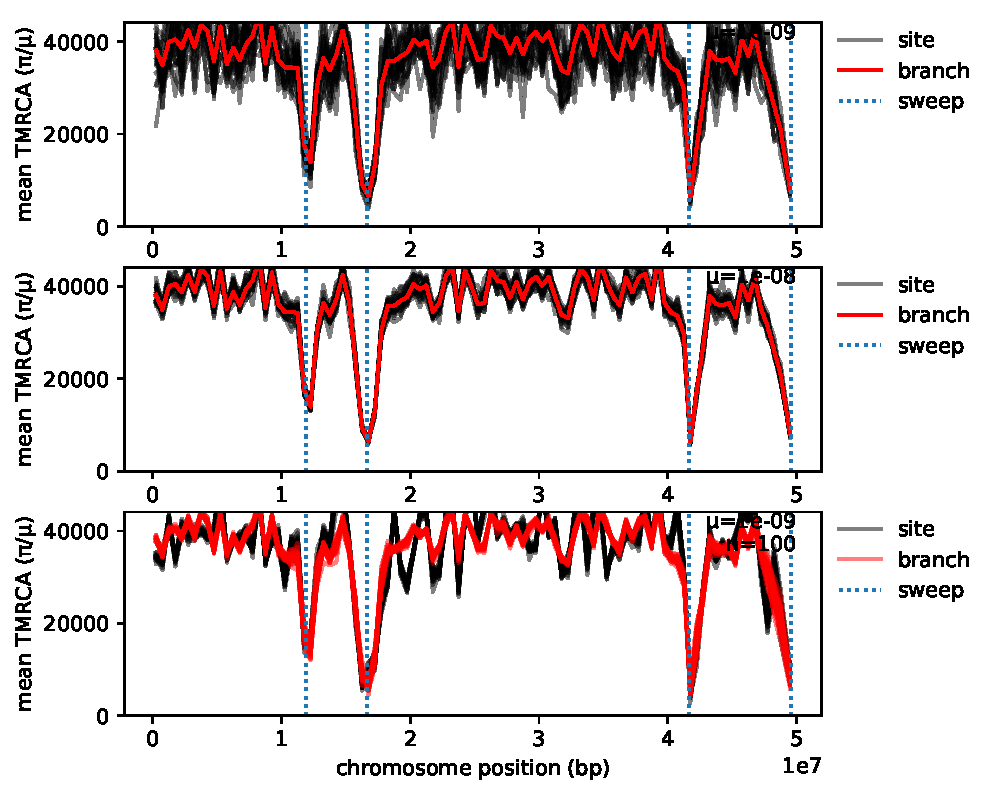
\includegraphics{{figures/swept.10000.765.1e-09.diversity}.pdf}
    \caption{
        As in Figure~\ref{fig:sweep_duality}, but in a population of size 10,000.
        \label{sfig:sweep_duality_10K}
    }
\end{figure}

\begin{figure}
    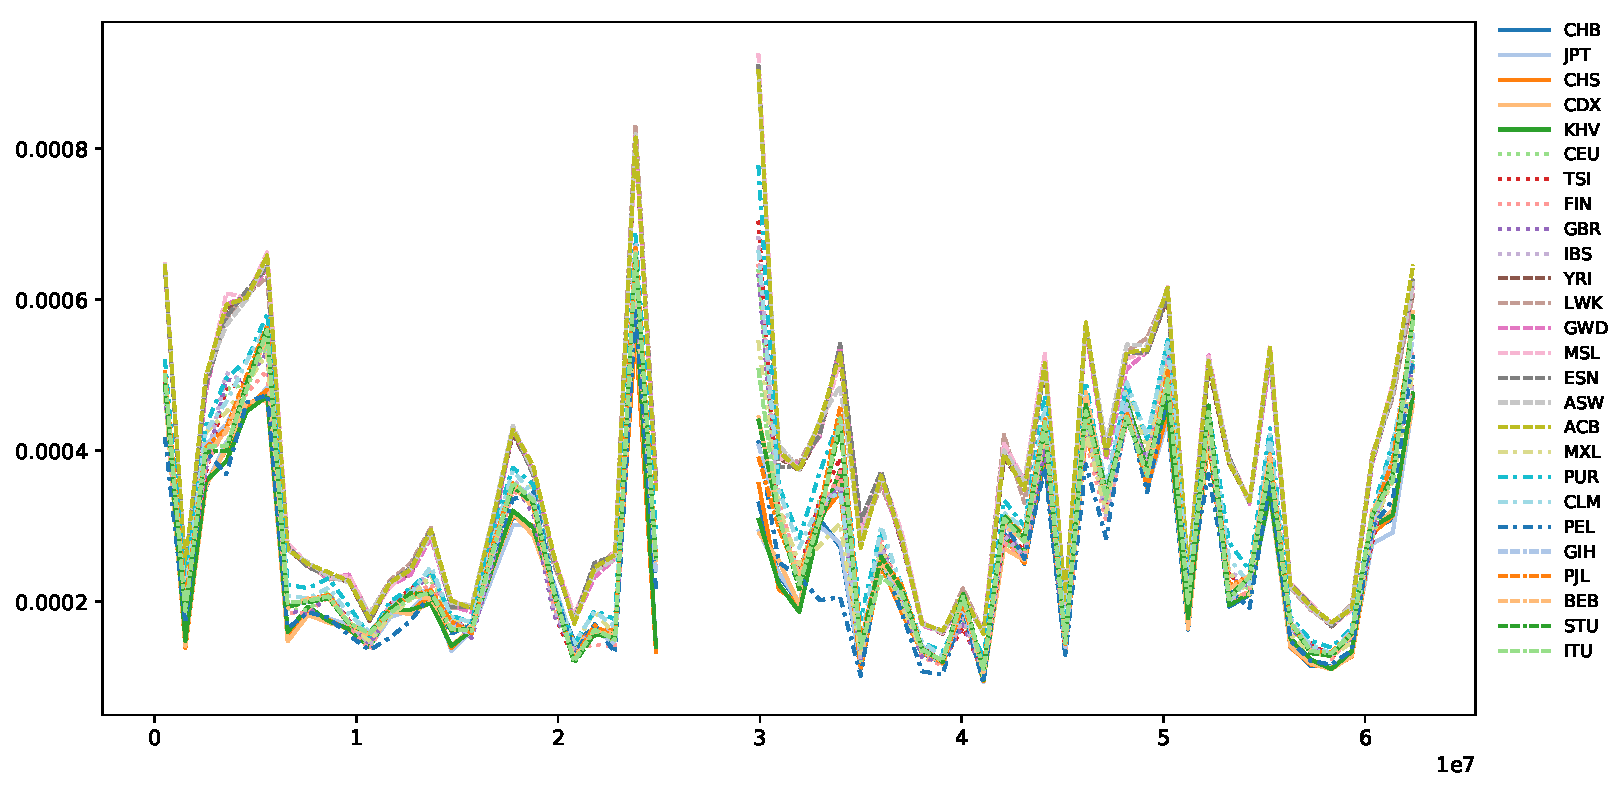
\includegraphics[width=\textwidth]{{figures/1kg/relate_chr20.site.1000000.diversity}.pdf}
    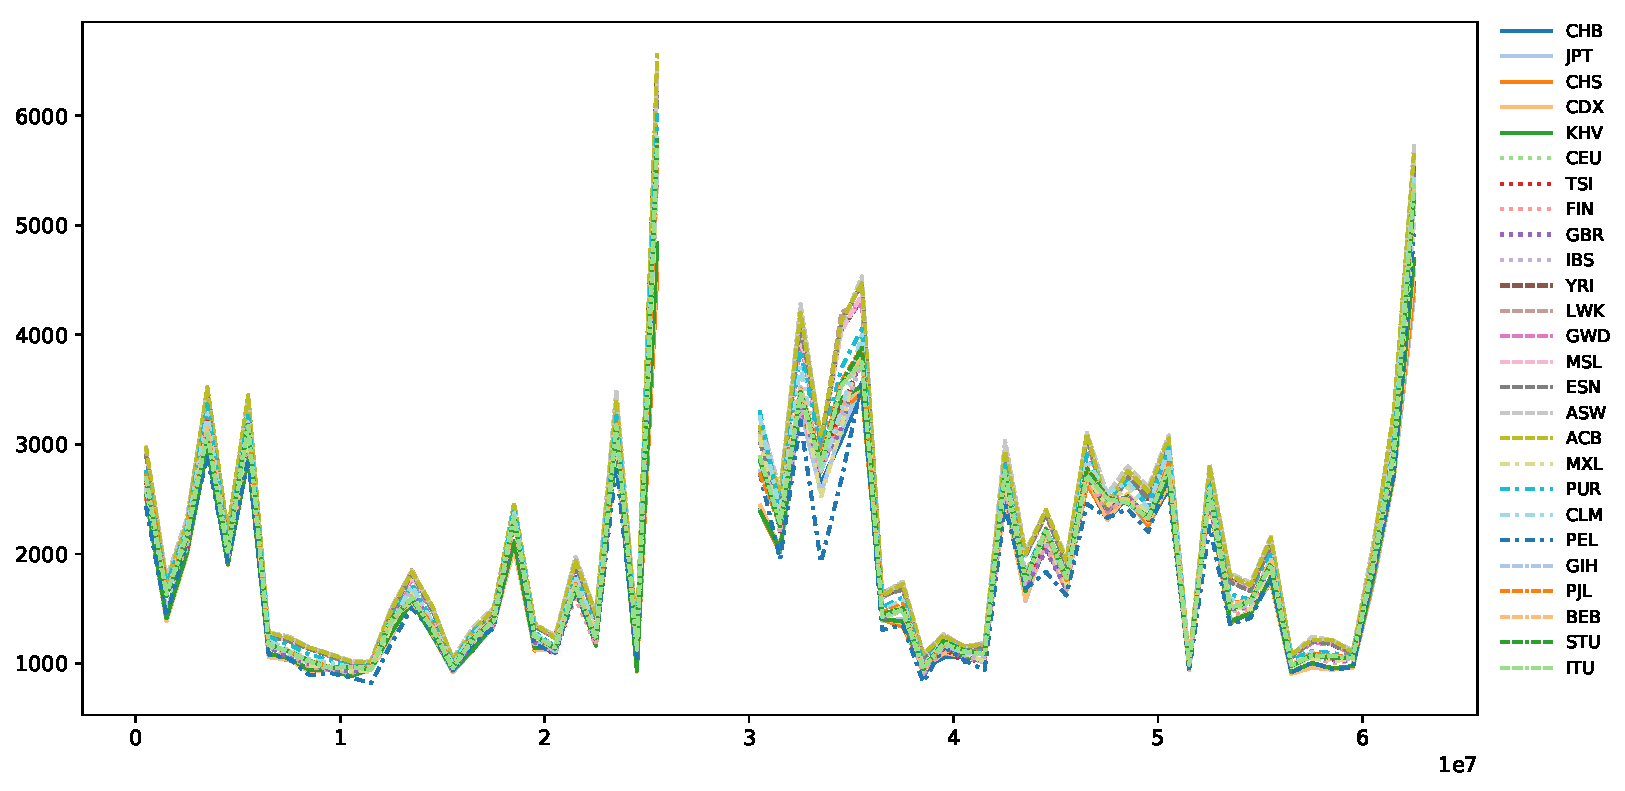
\includegraphics[width=\textwidth]{{figures/1kg/1kg_chr20.branch.1000000.diversity}.pdf}
    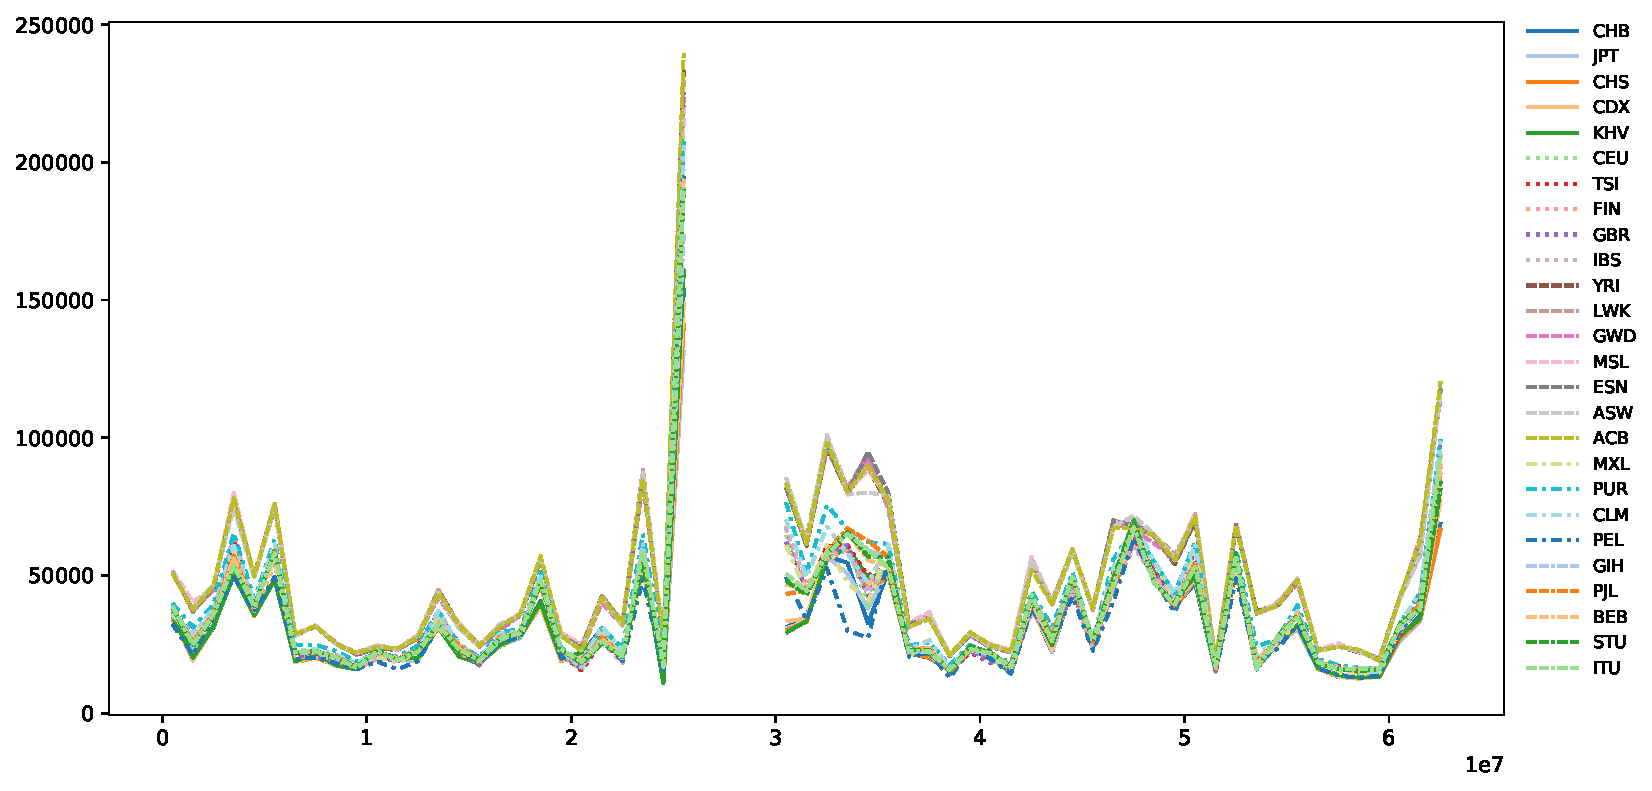
\includegraphics[width=\textwidth]{{figures/1kg/tgp_geva_chr20.branch.1000000.diversity}.pdf}
    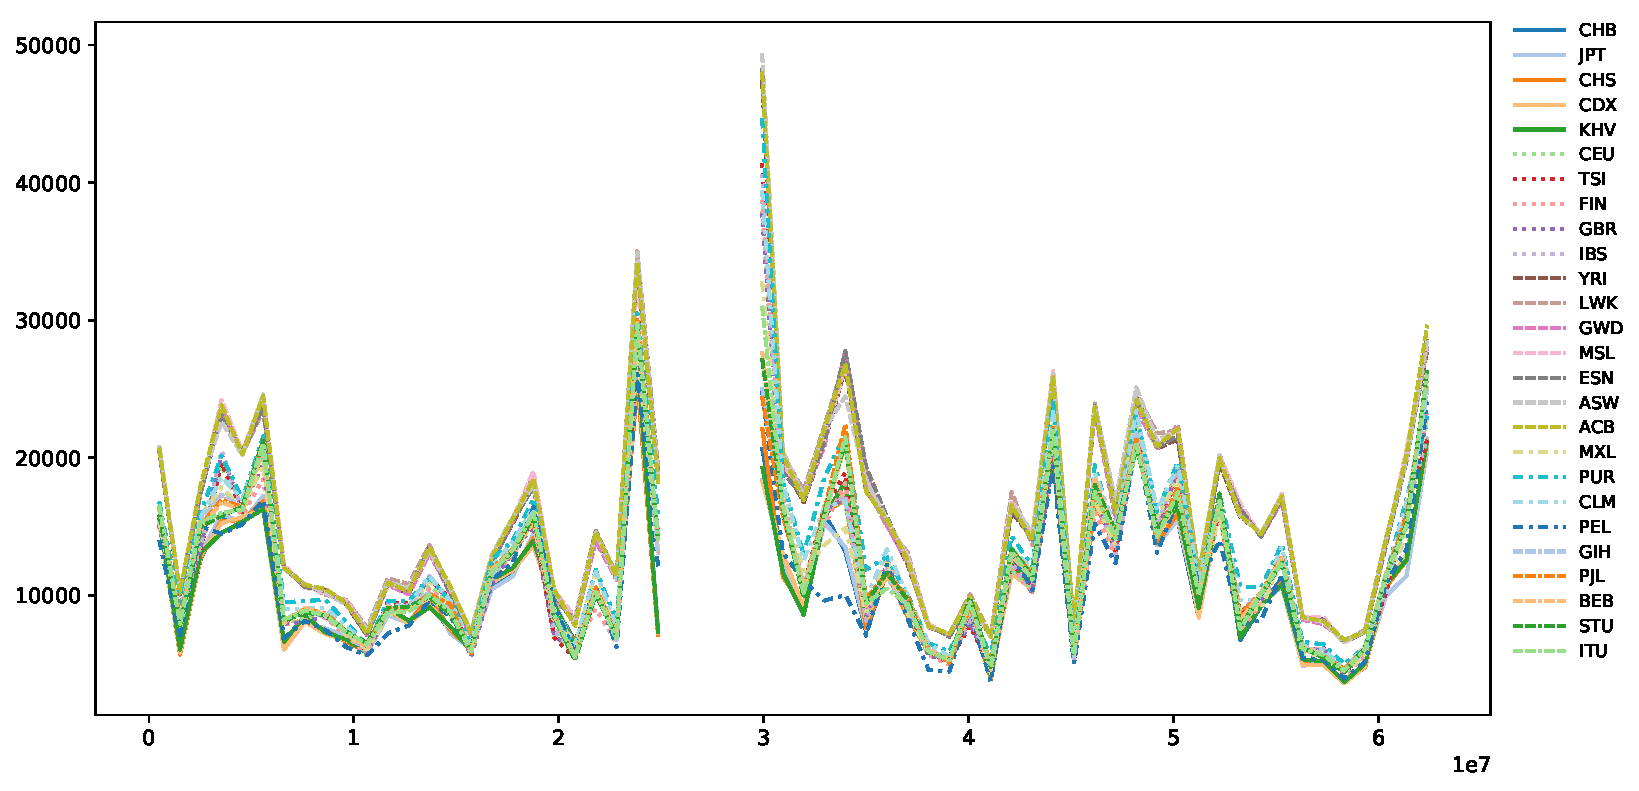
\includegraphics[width=\textwidth]{{figures/1kg/relate_chr20.branch.1000000.diversity}.pdf}
    \caption{
        \textbf{(top left)} Mean sequence diversity 
        in 1Mb windows along human chromosome 20 of the 1000 Genomes Project,
        and the dual branch statistic as calculated from tree sequences inferred by
        \textbf{(top right)} tsinfer,
        \textbf{(bottom left)} GEVA, and 
        \textbf{(bottom right)} Relate.
        \label{fig:chr20_full}
    }
\end{figure}



\end{document}


%%%%%%%%%%%%%%%%%%
\subsection*{Genomic PCA}

Let $G$ denote the genotype matrix, so that $G_{ja} \in \{0,1\}$
is the genotype of the $a^\text{th}$ individual
at the $j^\text{th}$ site, with `1` denoting the derived state
(we assume here biallelic markers).
Also let $P_j = (1/n) \sum_a G{ja}$ denote the vector of allele frequencies.
Then the \emph{genetic covariance} between samples $a$ and $b$ is
\begin{align*}
    C_{ab}
        &= \frac{1}{L} \sum_j (G_{ja} - P_j) (G_{jb} - P_j) . %  \\
        % &= \frac{1}{L} \left( (G - P \bone^T)^T (G - P \bone^T) \right)_{ab} .
\end{align*}
This can be computed by letting
$\iw_a = \delta_a$ and $\iw_b = \delta_b$
(these weights mark nodes above $a$ and $b$ respectively)
and $\iw_t = \bone / n$
(this weight gives the proportion of samples below each node).
Then, with
$f(\nw_a, \nw_b, \nw_t) = (\nw_a - \nw_t) (\nw_b - \nw_t)$,
we can compute the covariance as
\begin{align*}
    C_{ab} = \frac{1}{2} \bar \site(f, (\iw_a, \iw_b, \iw_t)) .
\end{align*}
This follows, including the factor of two,
because the summary function applied to the ancestral allele
at a site with derived allele frequencies $p_a$, $p_b$, and $p_t$
in sample $a$, sample $b$, and total, respectively, is
$f(1 - p_a, 1 - p_b, 1 - p_t) = f(p_a, p_b, p_t)$.

Computing the full covariance matrix for a large number of samples may be infeasible.
However, we can efficiently find $y^T C z$ for arbitrary vectors $y$ and $z$.
This works because if we set the initial weights to $y$,
then each allele's weight is equal to the sum of the entries of $y$
corresponding to samples carrying that allele.
Then, if we define
$f_{yz}(u, v, t) = (u - (\sum_a y_a) t) (v - (\sum_b z_b) t)$,
then
\begin{align} \label{eqn:yCz}
    \frac{1}{2} \bar \site(f_{yz}, (y, z, \iw_t))
        &= \frac{1}{L} \sum_j (\sum_a y_a G_{ja} - (\sum_a y_a) P_j)
                    (\sum_b z_b G_{jb} - (\sum_b z_b) P_j) \\
        &= y^T C z .
\end{align}

\plr{Hmph: to actually compute $Cz$ we need one weight vector for each sample, again.
    TODO: look up if you can do Krylov just by computing $y^t C z$ for a reasonable number of vectors.
    We could compute $Cz$ quickly if we could propagate down the tree:
    we'd have $(Cz)_a$ equal to the sum of the weights at all nodes \emph{above} $a$. }

Where does the signal from an eigenvector come from?
Let $y$ be an eigenvector of $C$ with eigenvalue $\lambda$, normalized so that $\|y\|^2 = 1$.
Since $Cy = \lambda y$,
we can write $1 = \sum_a y_a^2 = (1/\lambda) y^T C y$.
However, equation \eqref{eqn:yCz} gives $y^T C y$ as a sum over \emph{sites},
and thus distributes the variance in $G$ associated with $y$
across the tree sequence.
(This is true because of the singular value decomposition of $G$.)
